\documentclass{article}
\usepackage[a4paper, top=3cm, bottom=2.5cm, left=2.5cm, right=2.5cm]{geometry} % Ajuste de márgenes
\usepackage[spanish]{babel}
\usepackage[utf8]{inputenc}
\usepackage{tikz}
\usepackage{titling}
\usepackage{graphicx}
\usepackage{fancyhdr}
\usepackage{amsmath}
\usepackage{amssymb}
\usepackage{multicol}
\usepackage{cancel}
\usepackage{pgfplots}
\usepackage{float}
\usepackage{hyperref}
\pgfplotsset{compat=1.18}
\usepackage{titlesec} % Para personalizar títulos
\usepackage{tocloft}  % Para mejorar el índice
\usepackage{setspace} % Para controlar el espaciado

% Configuración de Fancyhdr para encabezados y pies de página
\pagestyle{fancy}
\fancyhf{}
\fancyhead[L]{
\includegraphics[width=2cm]{assets/logo-utp.png}}
\fancyhead[R]{\textbf{Mecánica Clásica}}

\fancyfoot[R]{\thepage} % Número de página alineado a la derecha

% Ajustes de espaciado entre párrafos y márgenes superiores
\setlength{\parskip}{1.5em}
\setlength{\parindent}{0pt}
\setlength{\headheight}{17.26935pt} % Altura del encabezado
\addtolength{\topmargin}{-2.26935pt} % Compensar el aumento de la altura del encabezado
\setlength{\textheight}{23cm}  % Ajusta el alto del texto

% Definición de comandos personalizados
\newcommand{\SubItem}[1]{
    {\setlength\itemindent{15pt} \item[-] #1}
}

% Título del documento con mejor control de espaciado
\title{
  
\includegraphics[width=5cm]{./assets/logo-utp.png} \\
  \vspace{1cm}
  \textbf{Universidad Tecnológica del Perú} \\
  \vspace{2cm}
  \textbf{Solucionario Sesión Integradora.} \\
  \vspace{1cm}
  \large \textbf{Para el curso de Mecánica Clásica.}
}
\author{
  \textbf{Luis Huatay Salcedo.} \\
  \texttt{hsluis4326@gmail.com} \\
  \texttt{U24218809 - 24229} \\
  \textbf{Cristian Miguel Cristóbal Blas.} \\
}


\begin{document}
\maketitle
\thispagestyle{empty}
\begin{center}
  Mg. Jonathan Joas Zapata Campos.  
\end{center}
\restoregeometry

\newpage

% \begin{center}
%   \textbf{\Large Índice}
% \end{center}
% \vspace{0.5cm} % Espacio entre título y contenido

% \begin{spacing}{1.15} % Espaciado personalizado para mayor legibilidad
%   \noindent
%   \begin{enumerate}
%     \item Introducción
%   %   \item Problemática
%   %   \item Objetivo general
%   %   \begin{enumerate}
%   %     \item Objetivos específicos
%   %   \end{enumerate}
%   %   \item Términos estadísticos
%   %   \item Recolección de información
%     \end{enumerate}
% \end{spacing}

% \newpage
% \vspace*{\fill}
% \section{Introducción}
% La aleatoriedad es un concepto fundamental en la teoría de la probabilidad y la estadística, en la informática, ciencias de la computación, criptografía, etc. Hoy en día nuestras cuentas bancarias, códigos de seguridad y datos personales dependen de la aleatoriedad para permanecer seguros. Para esto existen muchos algoritmos matemáticos que pretenden dar una solución a esto en la generación de números aleatorios. Sin embargo es matemáticamente imposible para una computadora crear un número verdaderamente aleatorio.

% Sin emabrgo, existen medios físicos que pueden ser utilizados para generar aleatoriedad, en lo que los expertos llaman \textit{entropía}. La entropía es una medida de la incertidumbre o el desorden en un sistema. En el contexto de la generación de números aleatorios, la entropía se refiere a la cantidad de información impredecible que se puede extraer de un sistema físico. Cuanto más impredecible sea el sistema, mayor será su entropía.

% Es aquí donde entra en juego el Strandbeest \cite{strandbeest2024}, una obra maestra de la ingeniería y el arte creada por el artista e ingeniero Theo Jansen Strandbeest. El Strandbeest es una criatura mecánica que camina utilizando energía eólica, y su diseño se basa en principios de la mecánica clásica. La idea detrás de este proyecto es utilizar el movimiento del Strandbeest para generar números aleatorios a partir de la entropía eólica.

% \vspace*{\fill}

% \newpage



% \newpage

% \bibliographystyle{plain} % Estilo (APA, IEEE, etc.)
% \bibliography{referencias} % Nombre del archivo .bib (sin extensión)  \printbibliography

\section{Problema 1}

\begin{figure}[ht!]
  \centering
  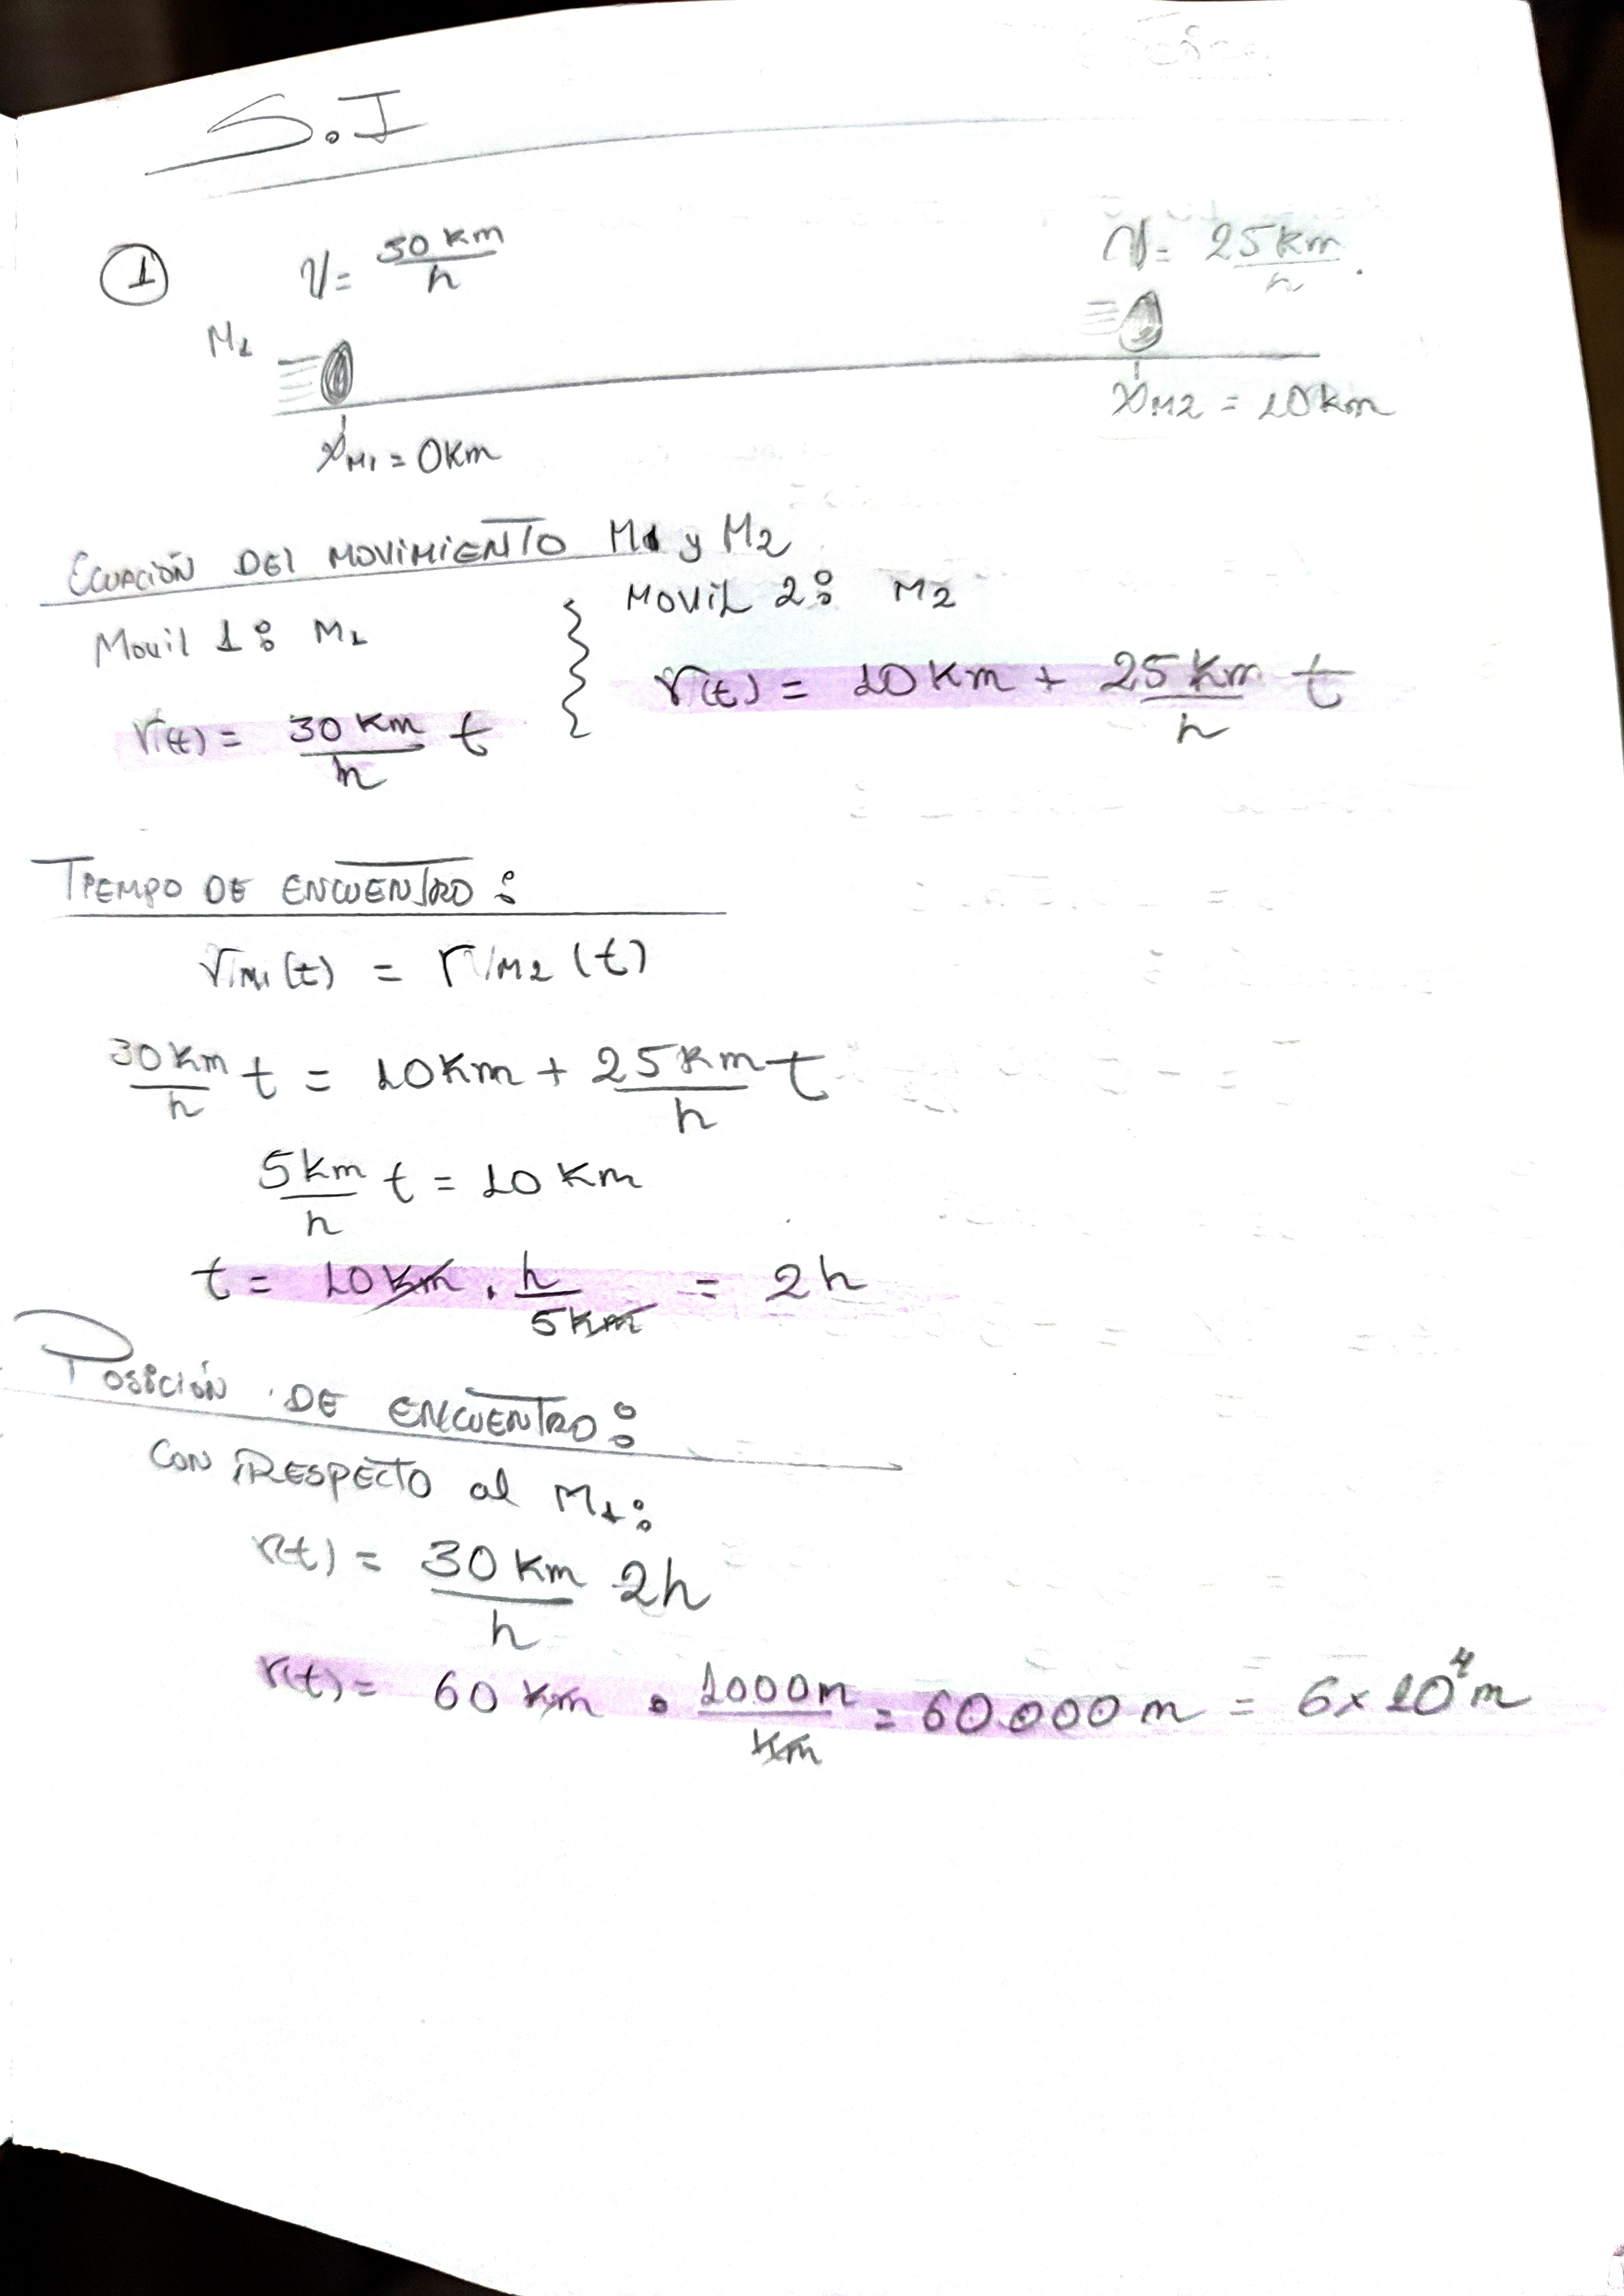
\includegraphics[width=0.9\textwidth]{assets/11.jpg}
  \label{fig:example_image1}
\end{figure}

\newpage

\section{Problema 2}

\begin{figure}[ht!]
  \centering
  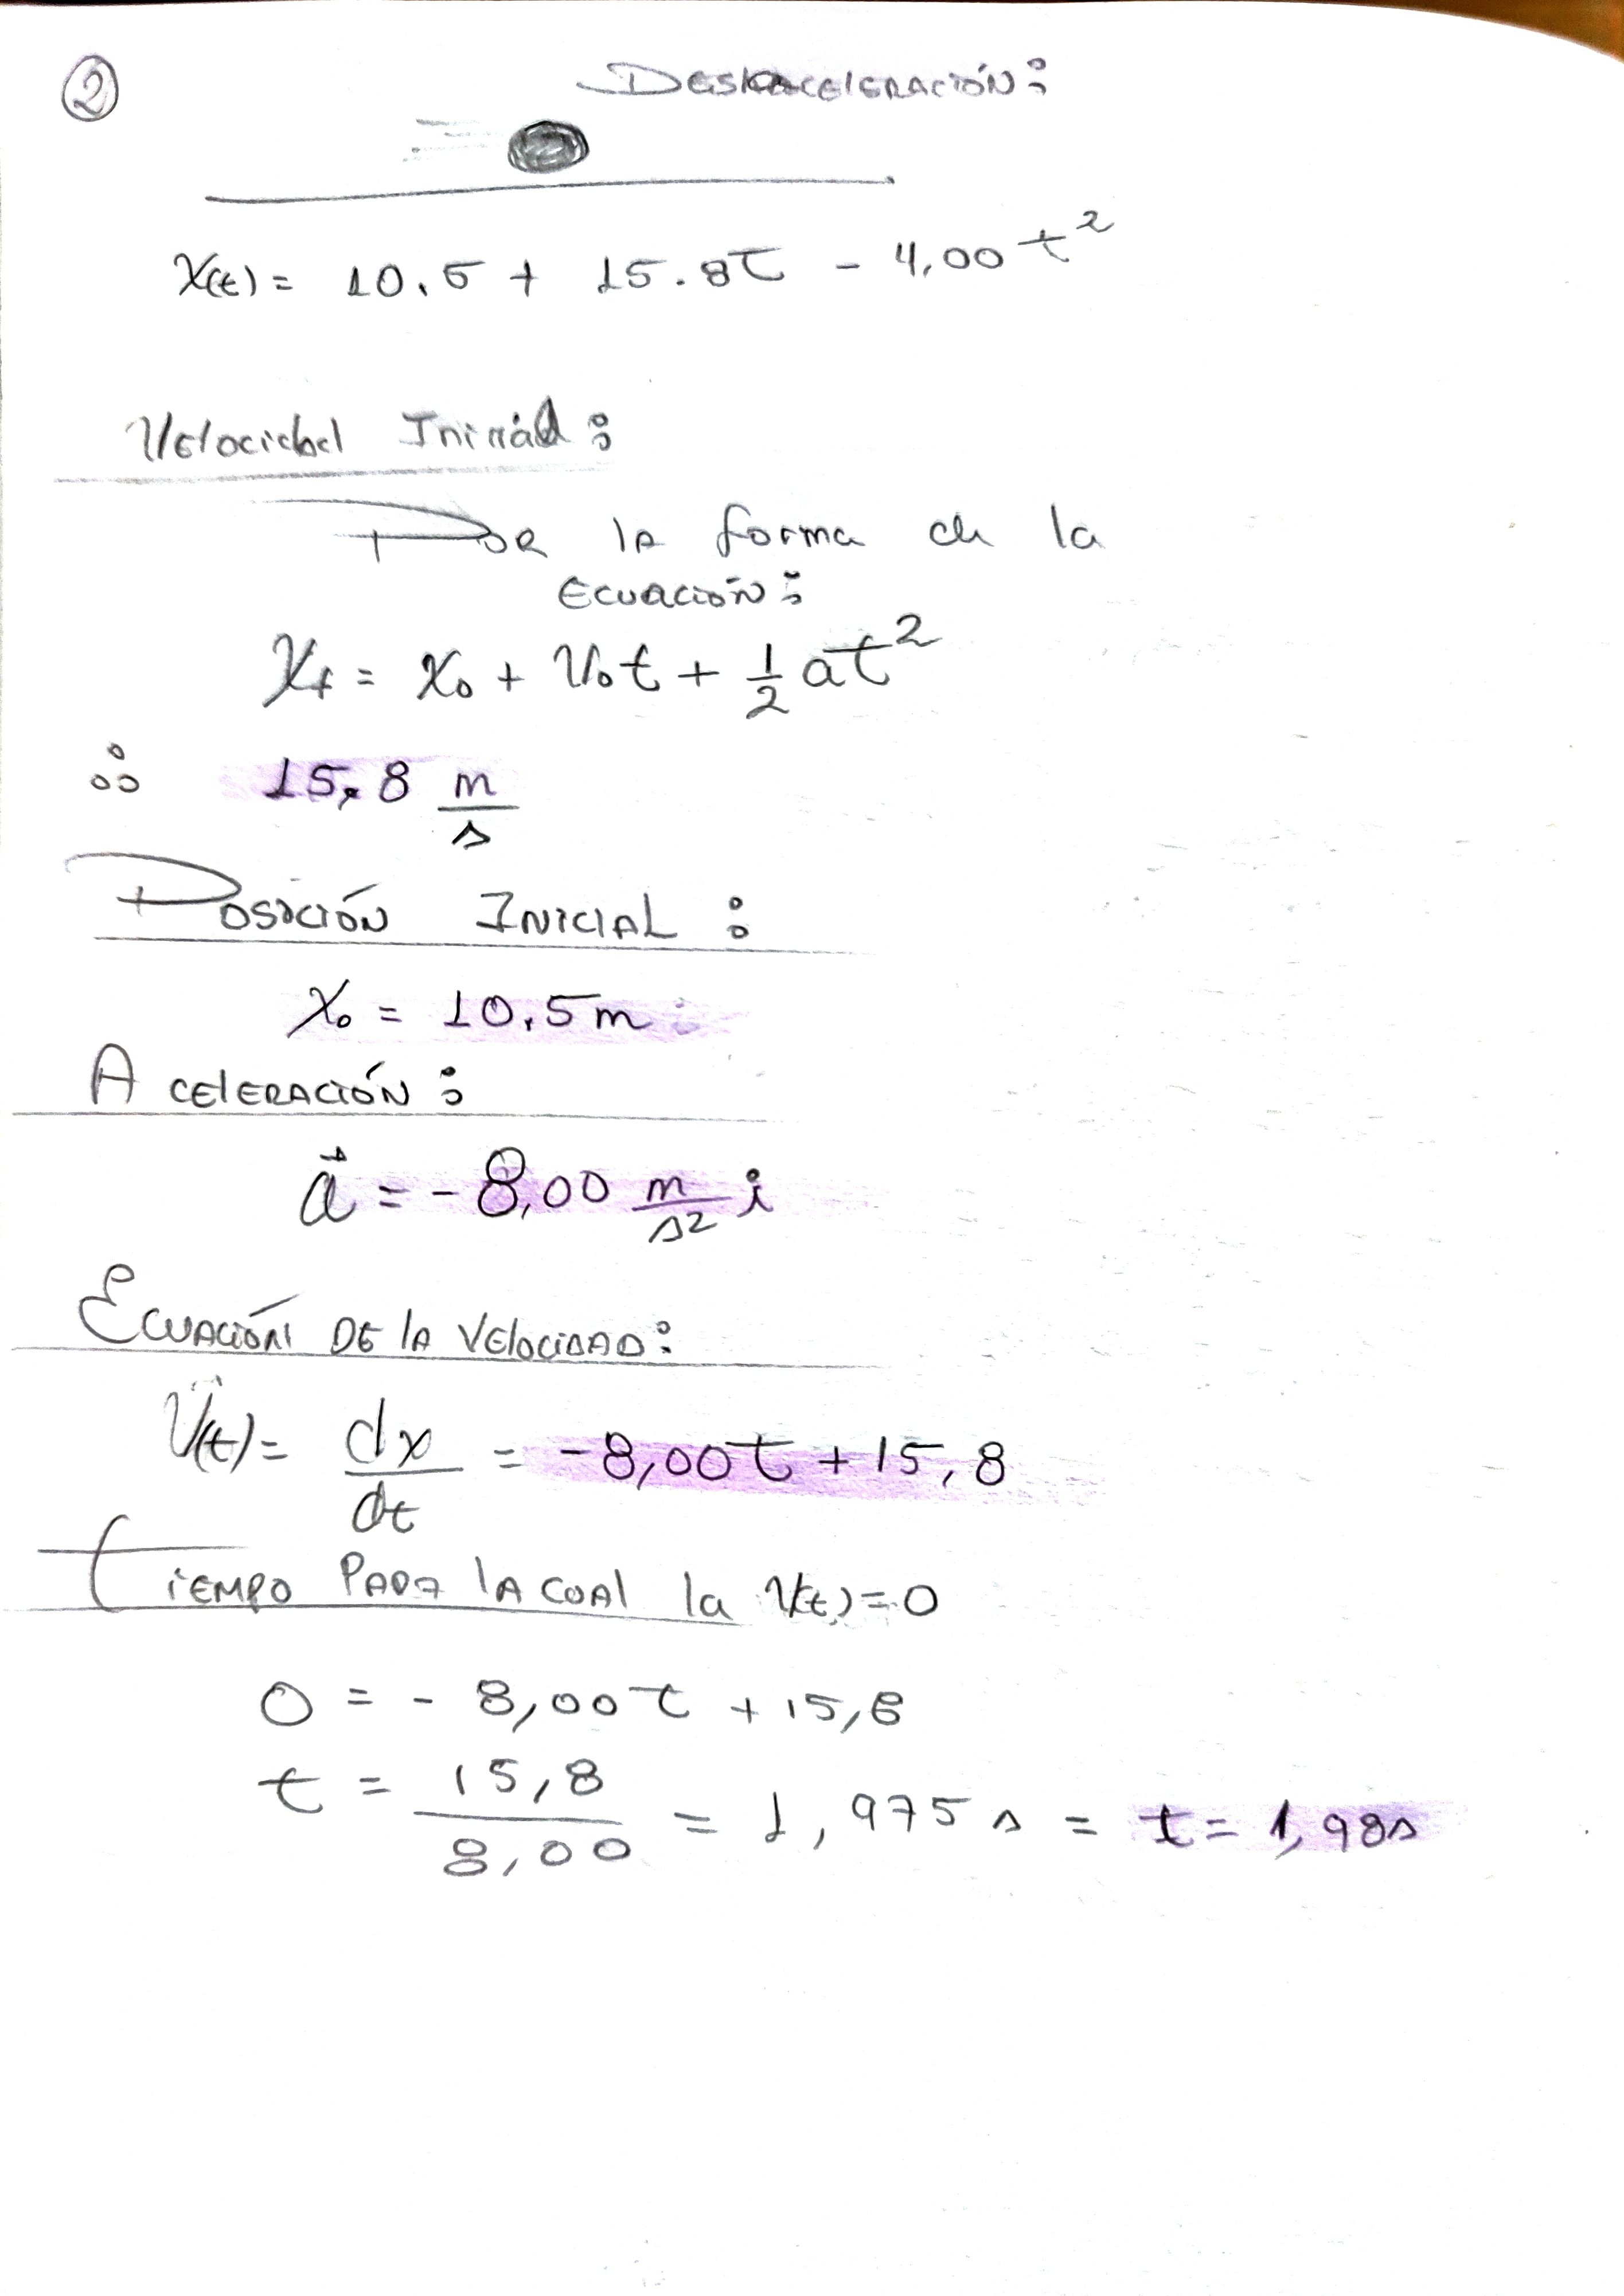
\includegraphics[width=0.9\textwidth]{assets/2.jpg}
  \label{fig:example_image2}
\end{figure}

\section{Problema 3}

\begin{figure}[H]
  \centering
  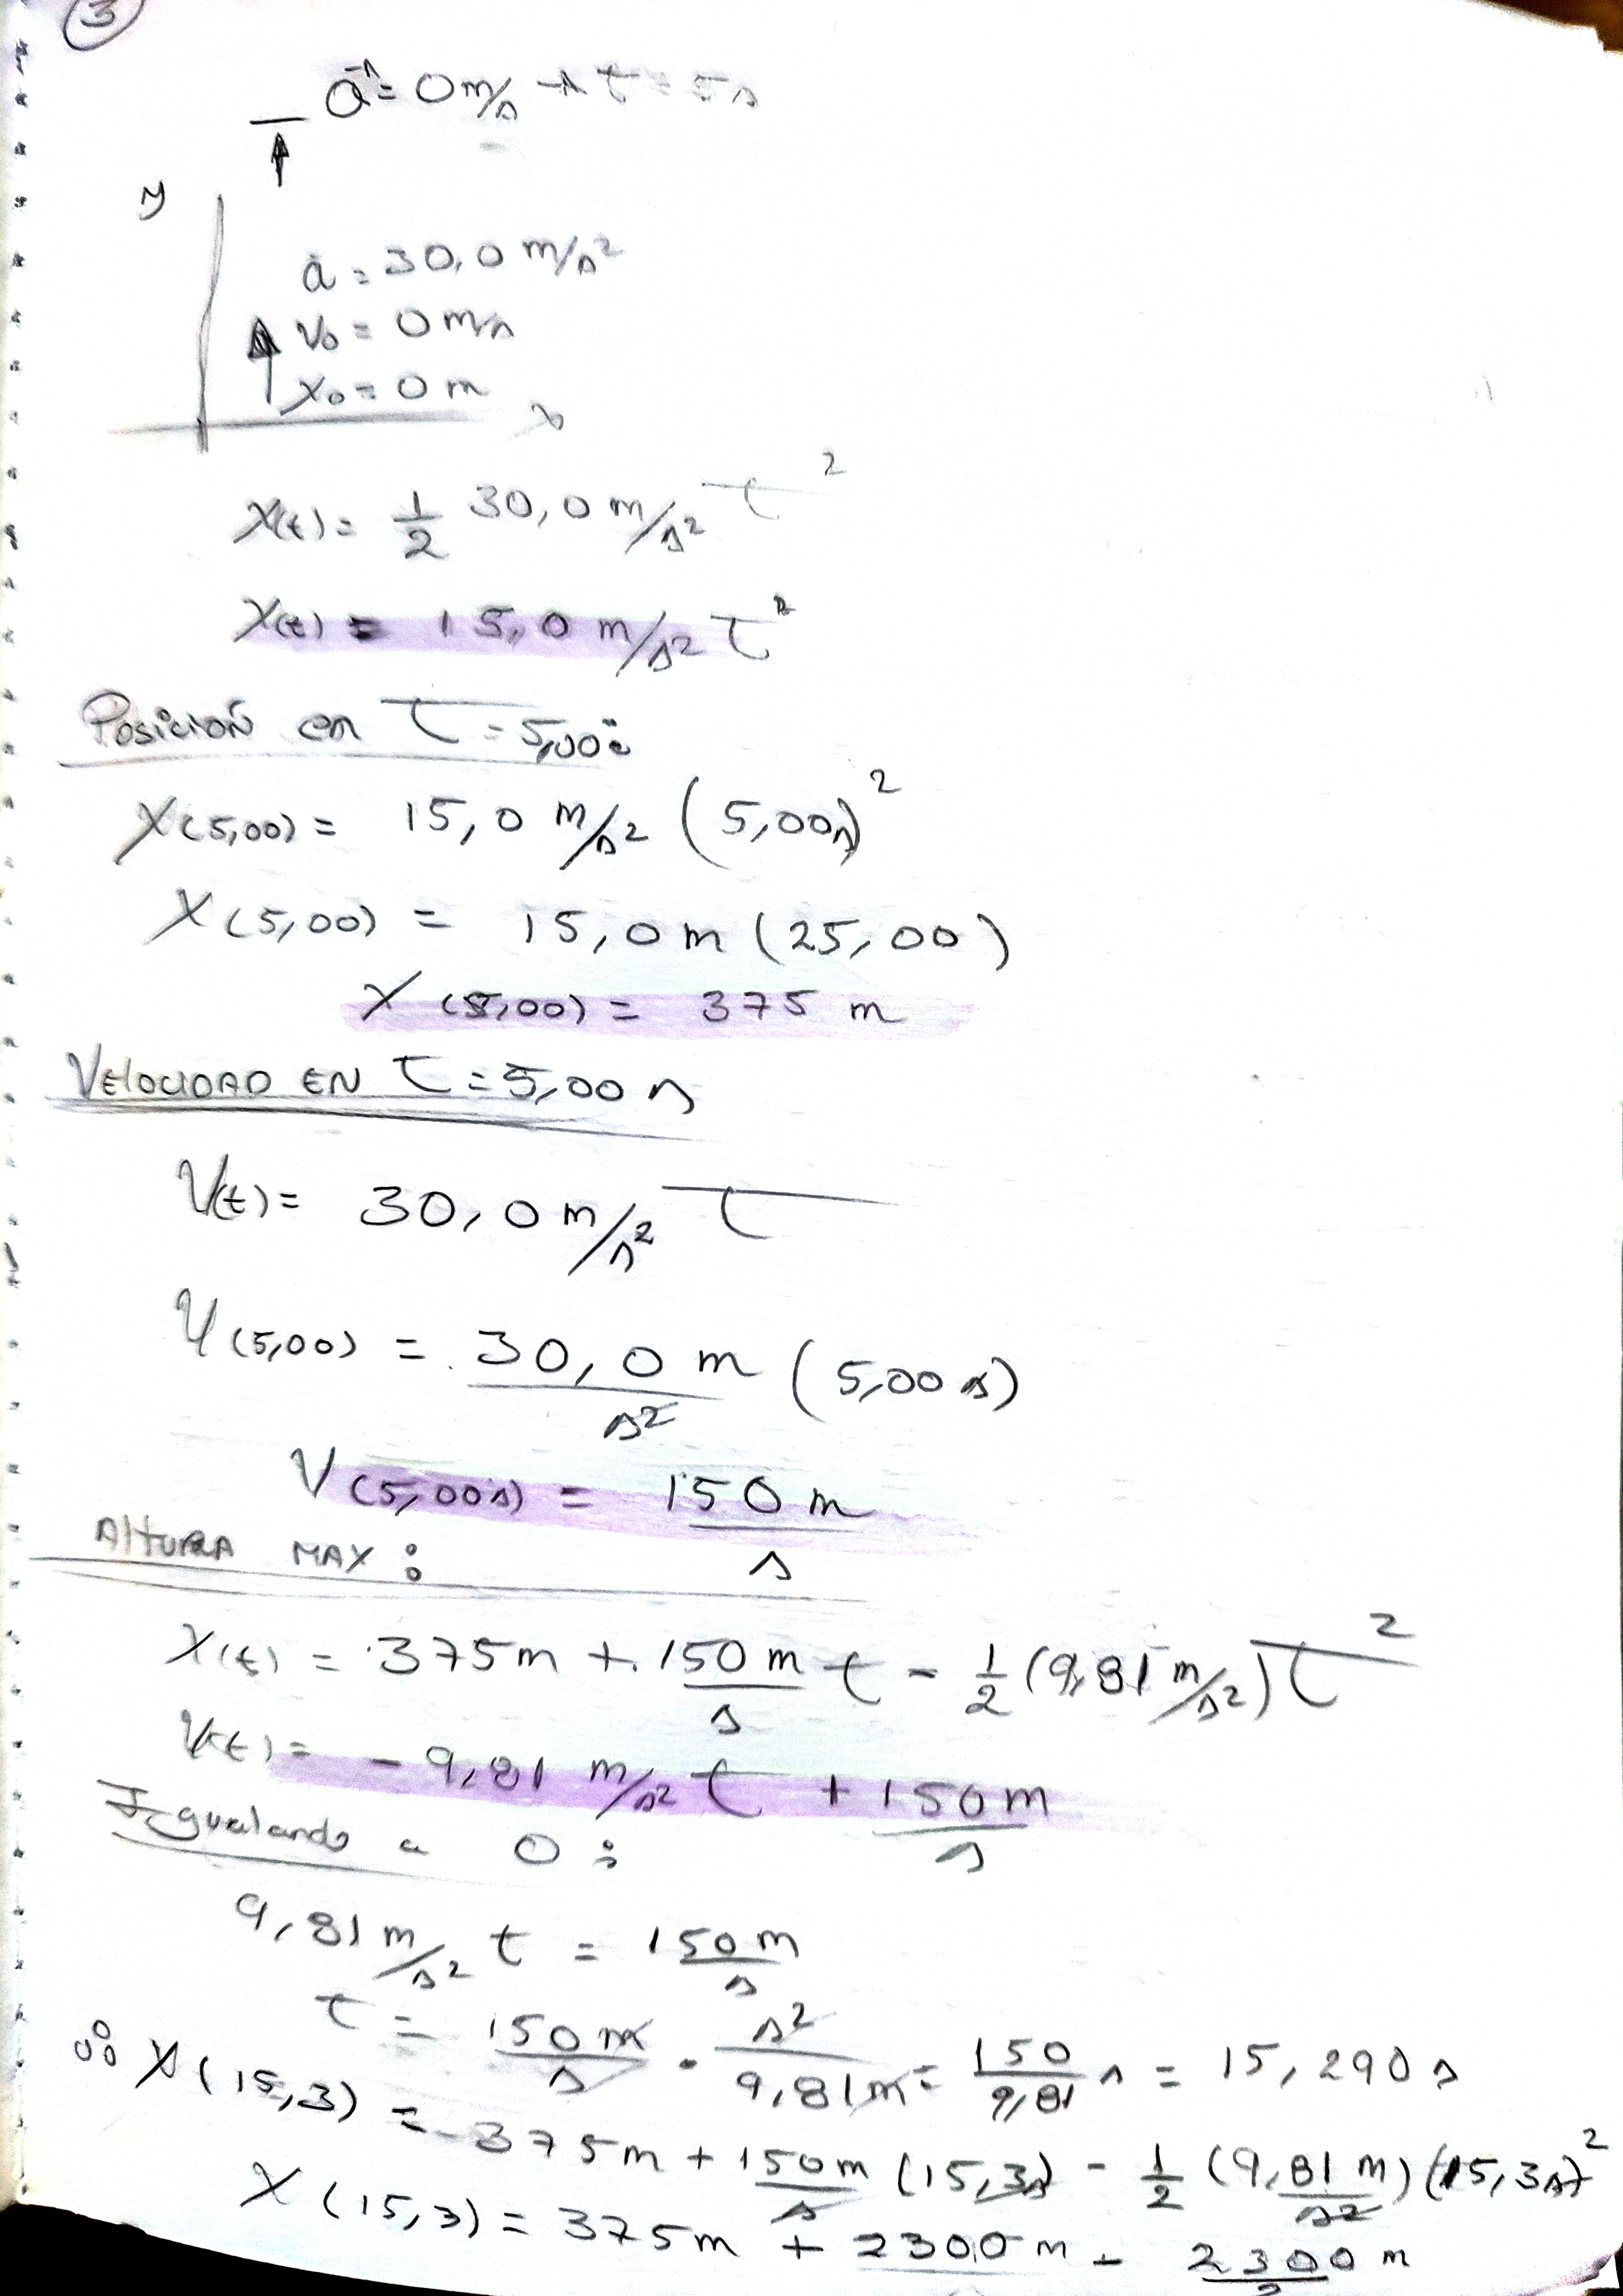
\includegraphics[width=0.9\textwidth]{assets/3.jpg}
  \label{fig:example_image3}
\end{figure}

\begin{figure}[H]
  \centering
  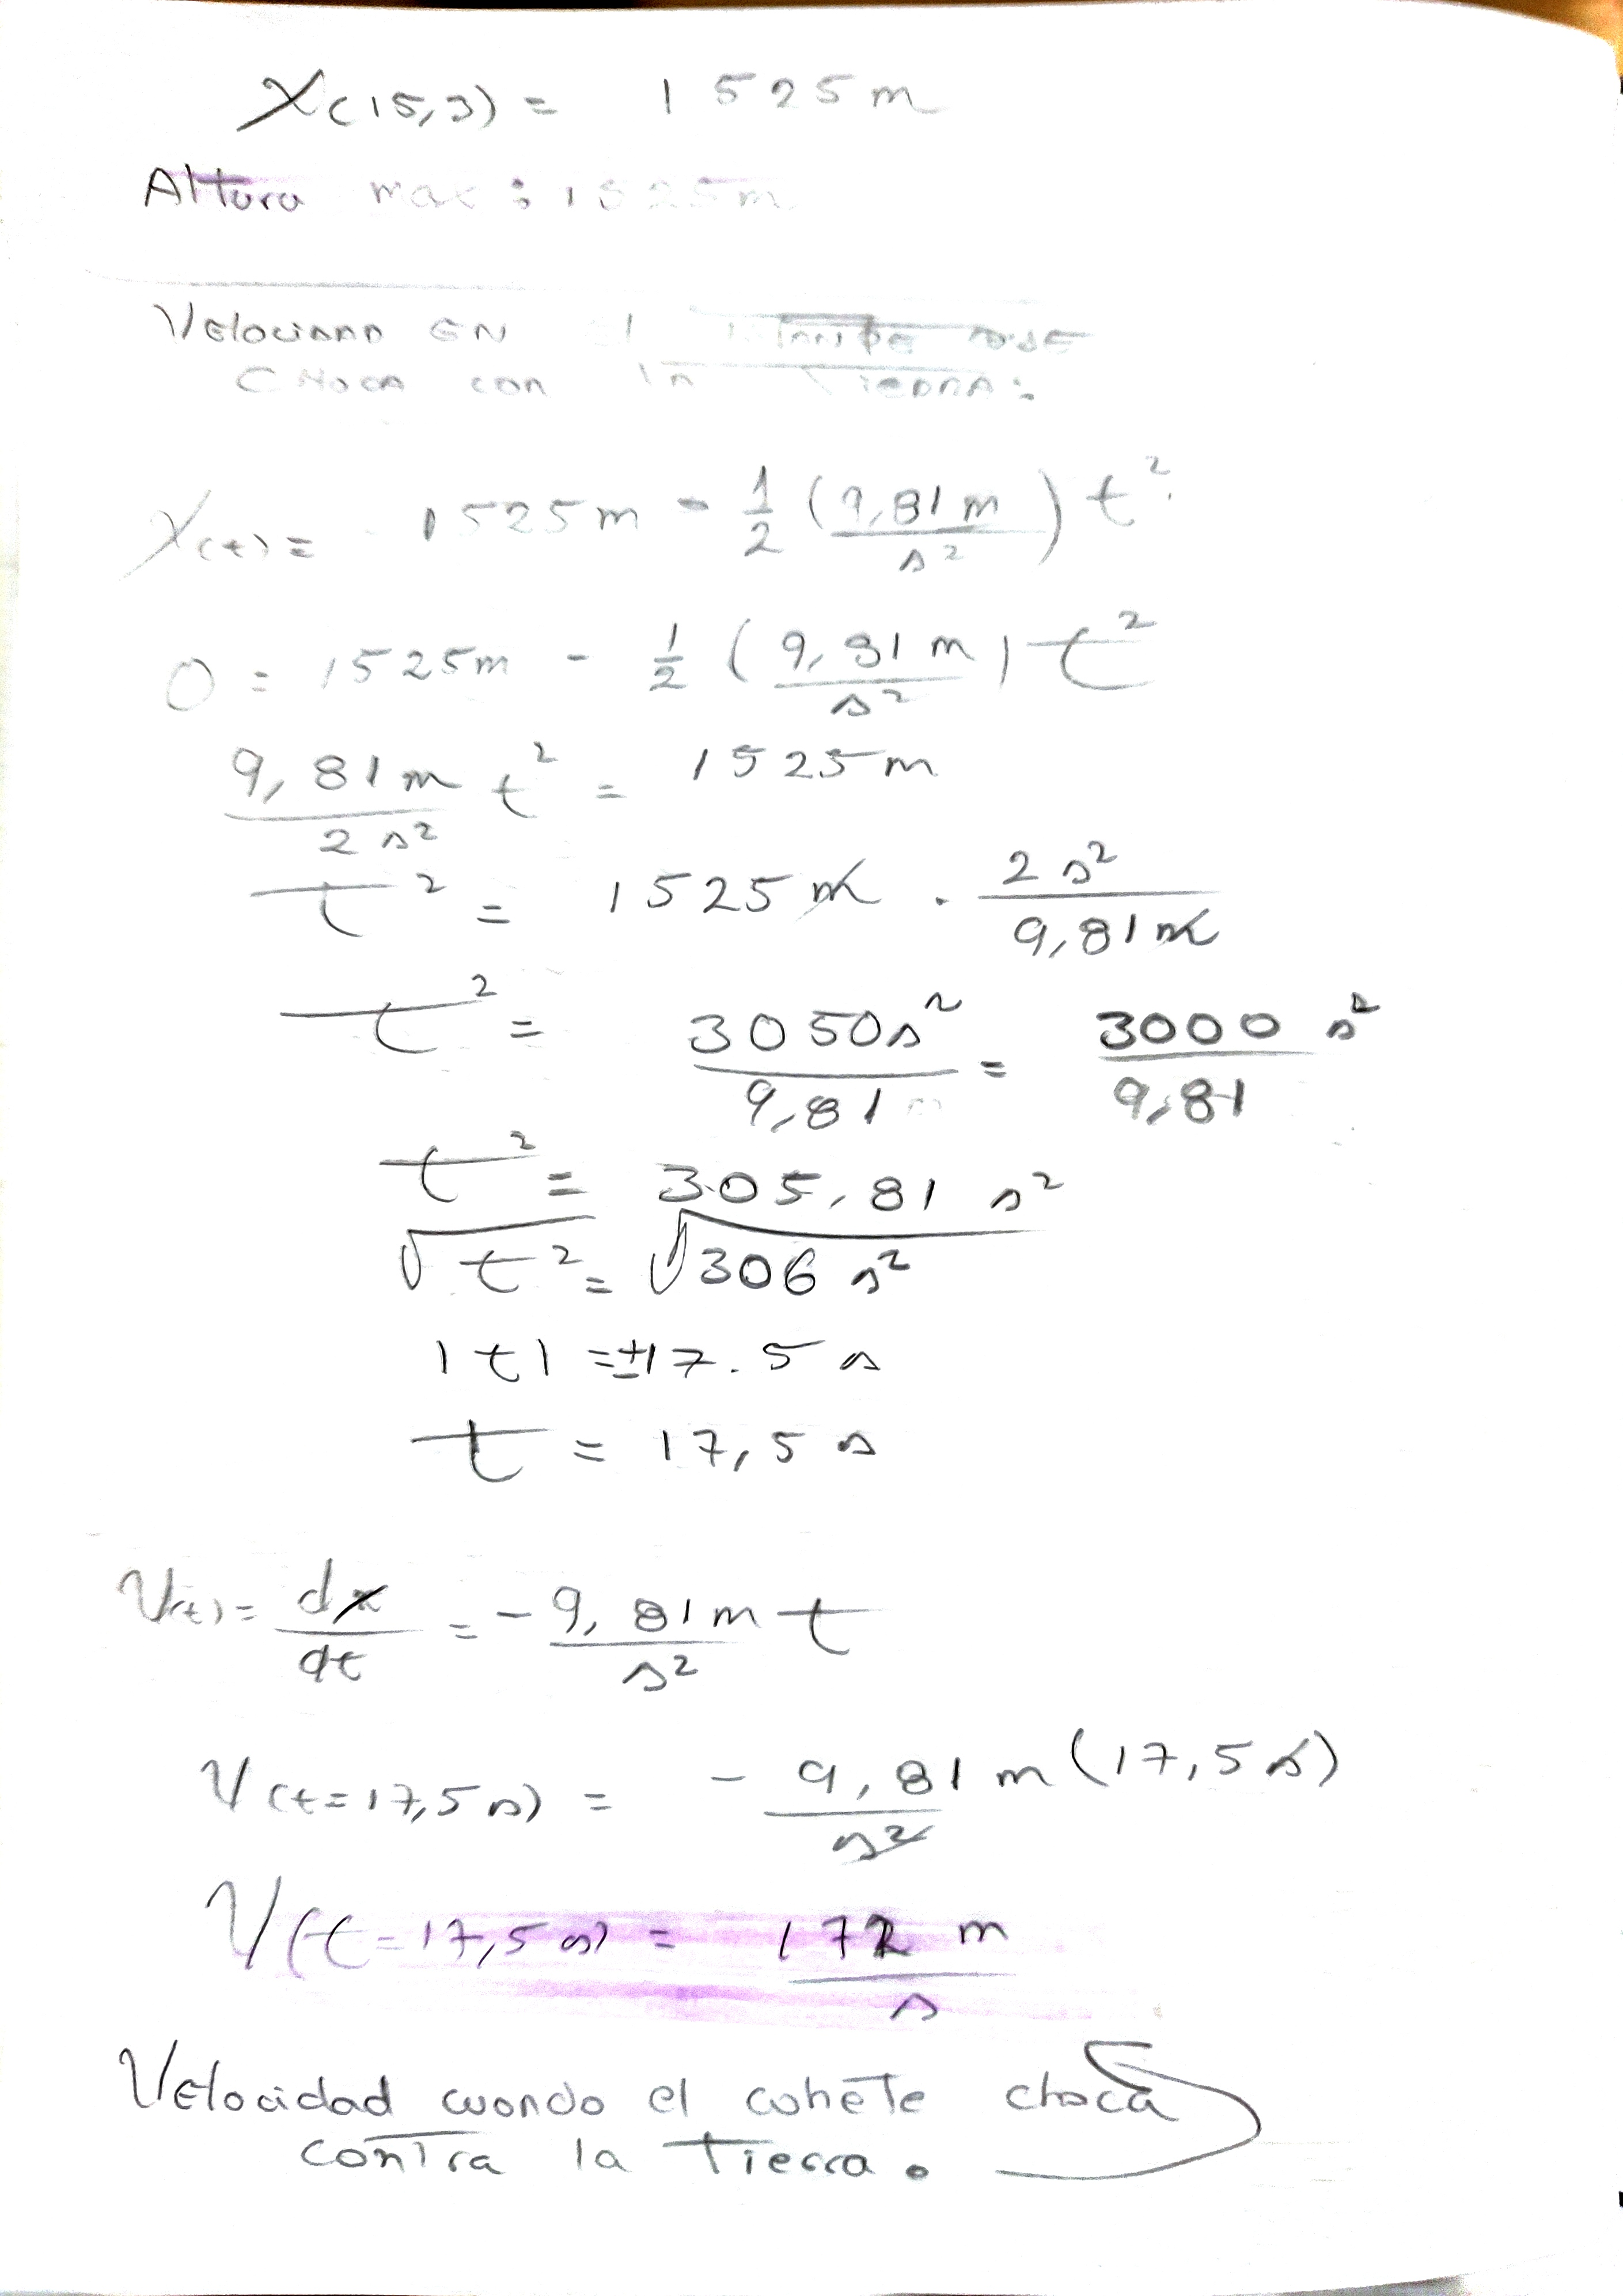
\includegraphics[width=0.9\textwidth]{assets/32.jpg}
  \label{fig:example_image32}
\end{figure}

\newpage
\section{Problema 4}
\begin{figure}[H]
  \centering
  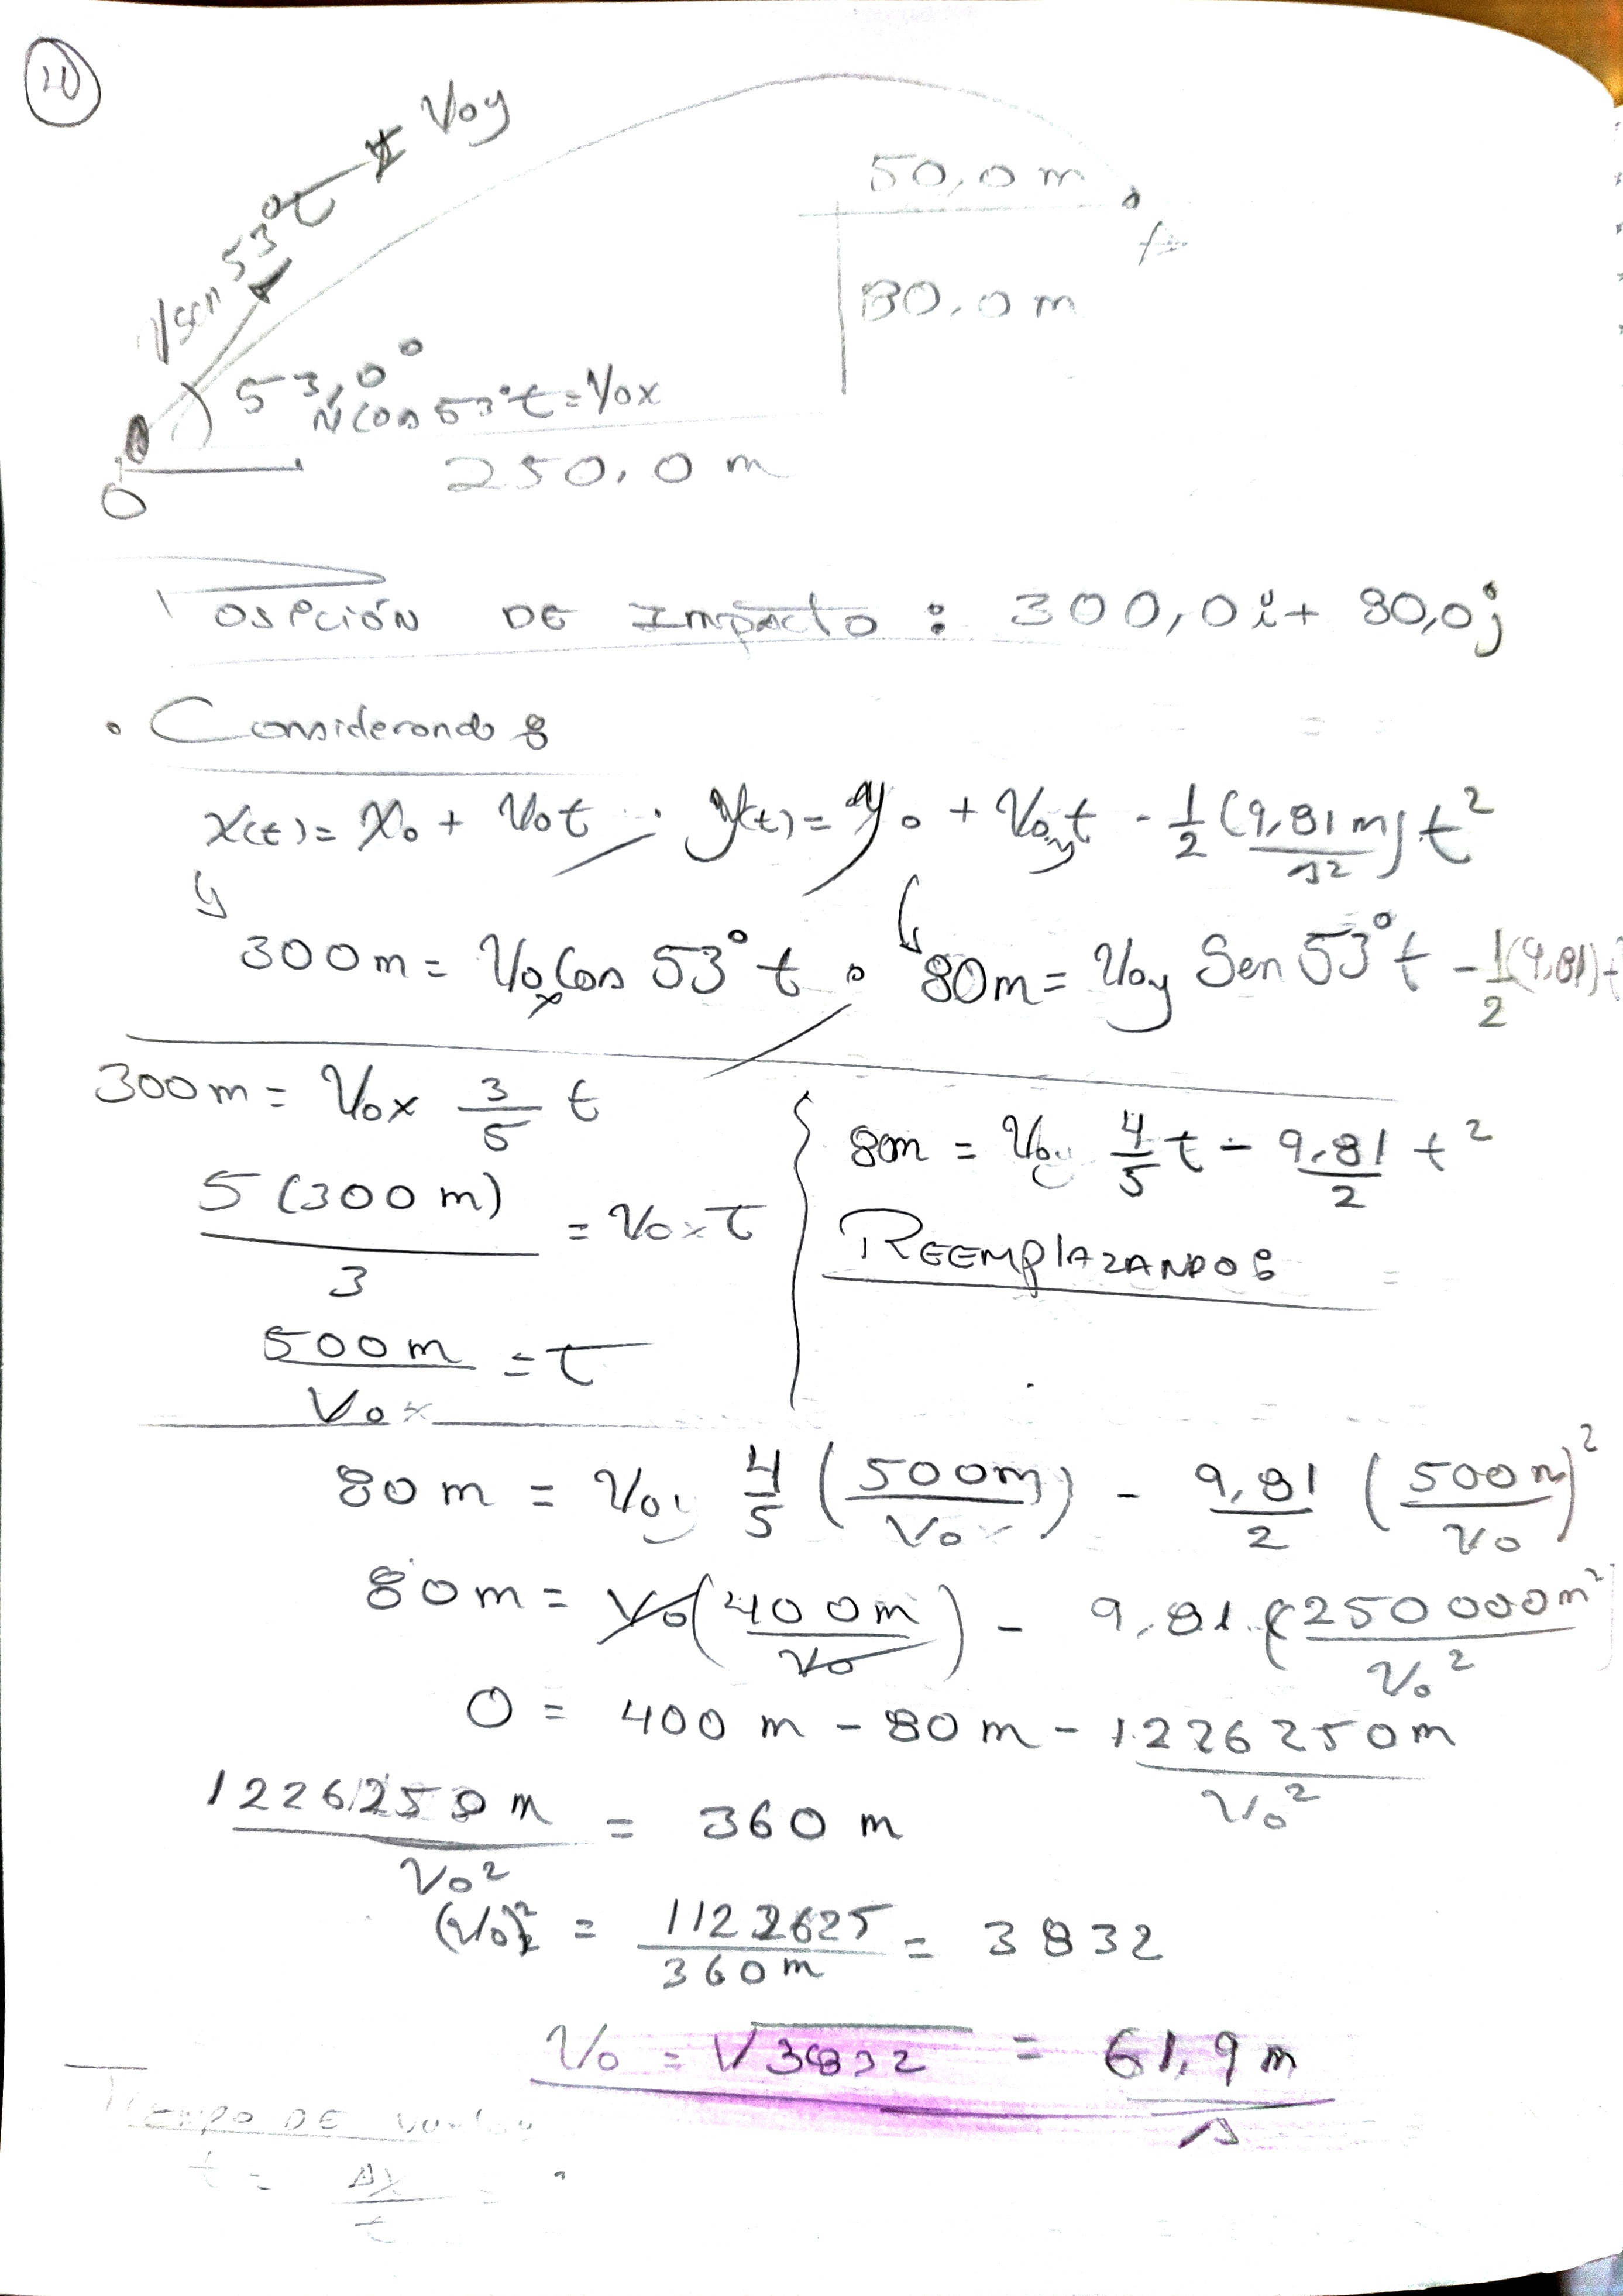
\includegraphics[width=0.9\textwidth]{assets/4.jpg}
  \label{fig:example_image4}
\end{figure}

\begin{figure}[H]
  \centering
  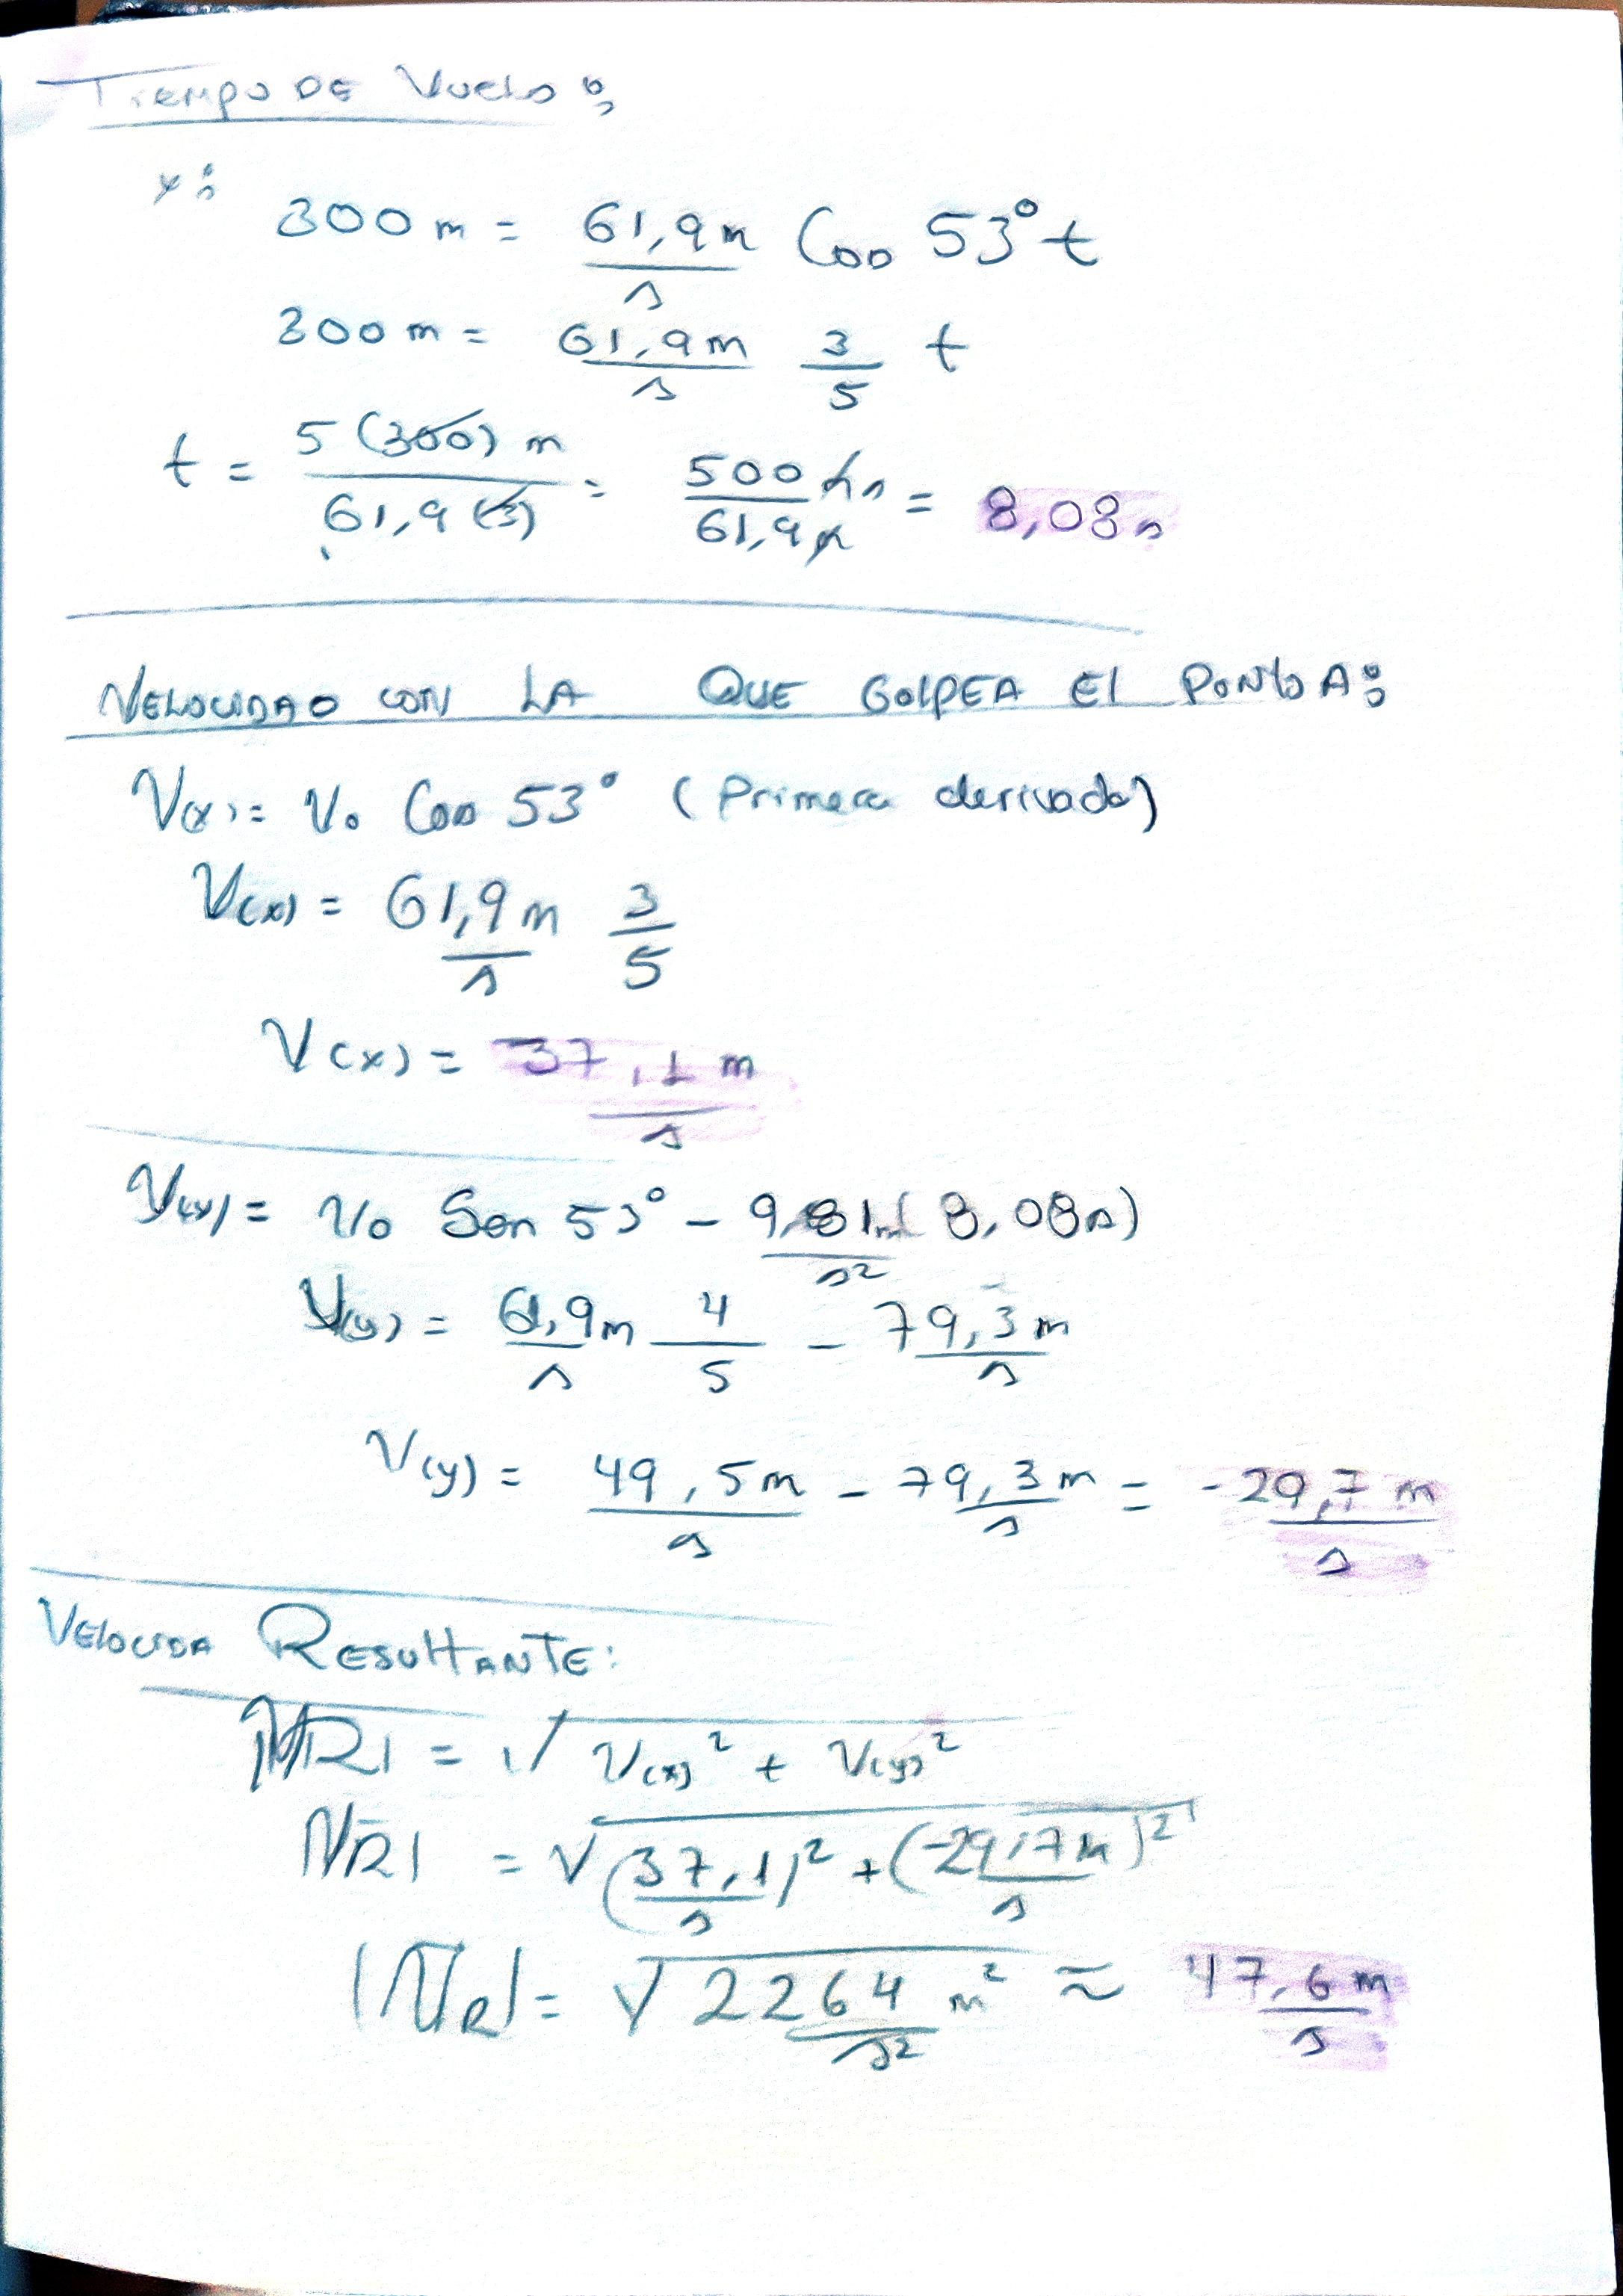
\includegraphics[width=0.9\textwidth]{assets/42.jpg}
  \label{fig:example_image42}
\end{figure}

\newpage
\section{Problema 5}
\begin{figure}[H]
  \centering
  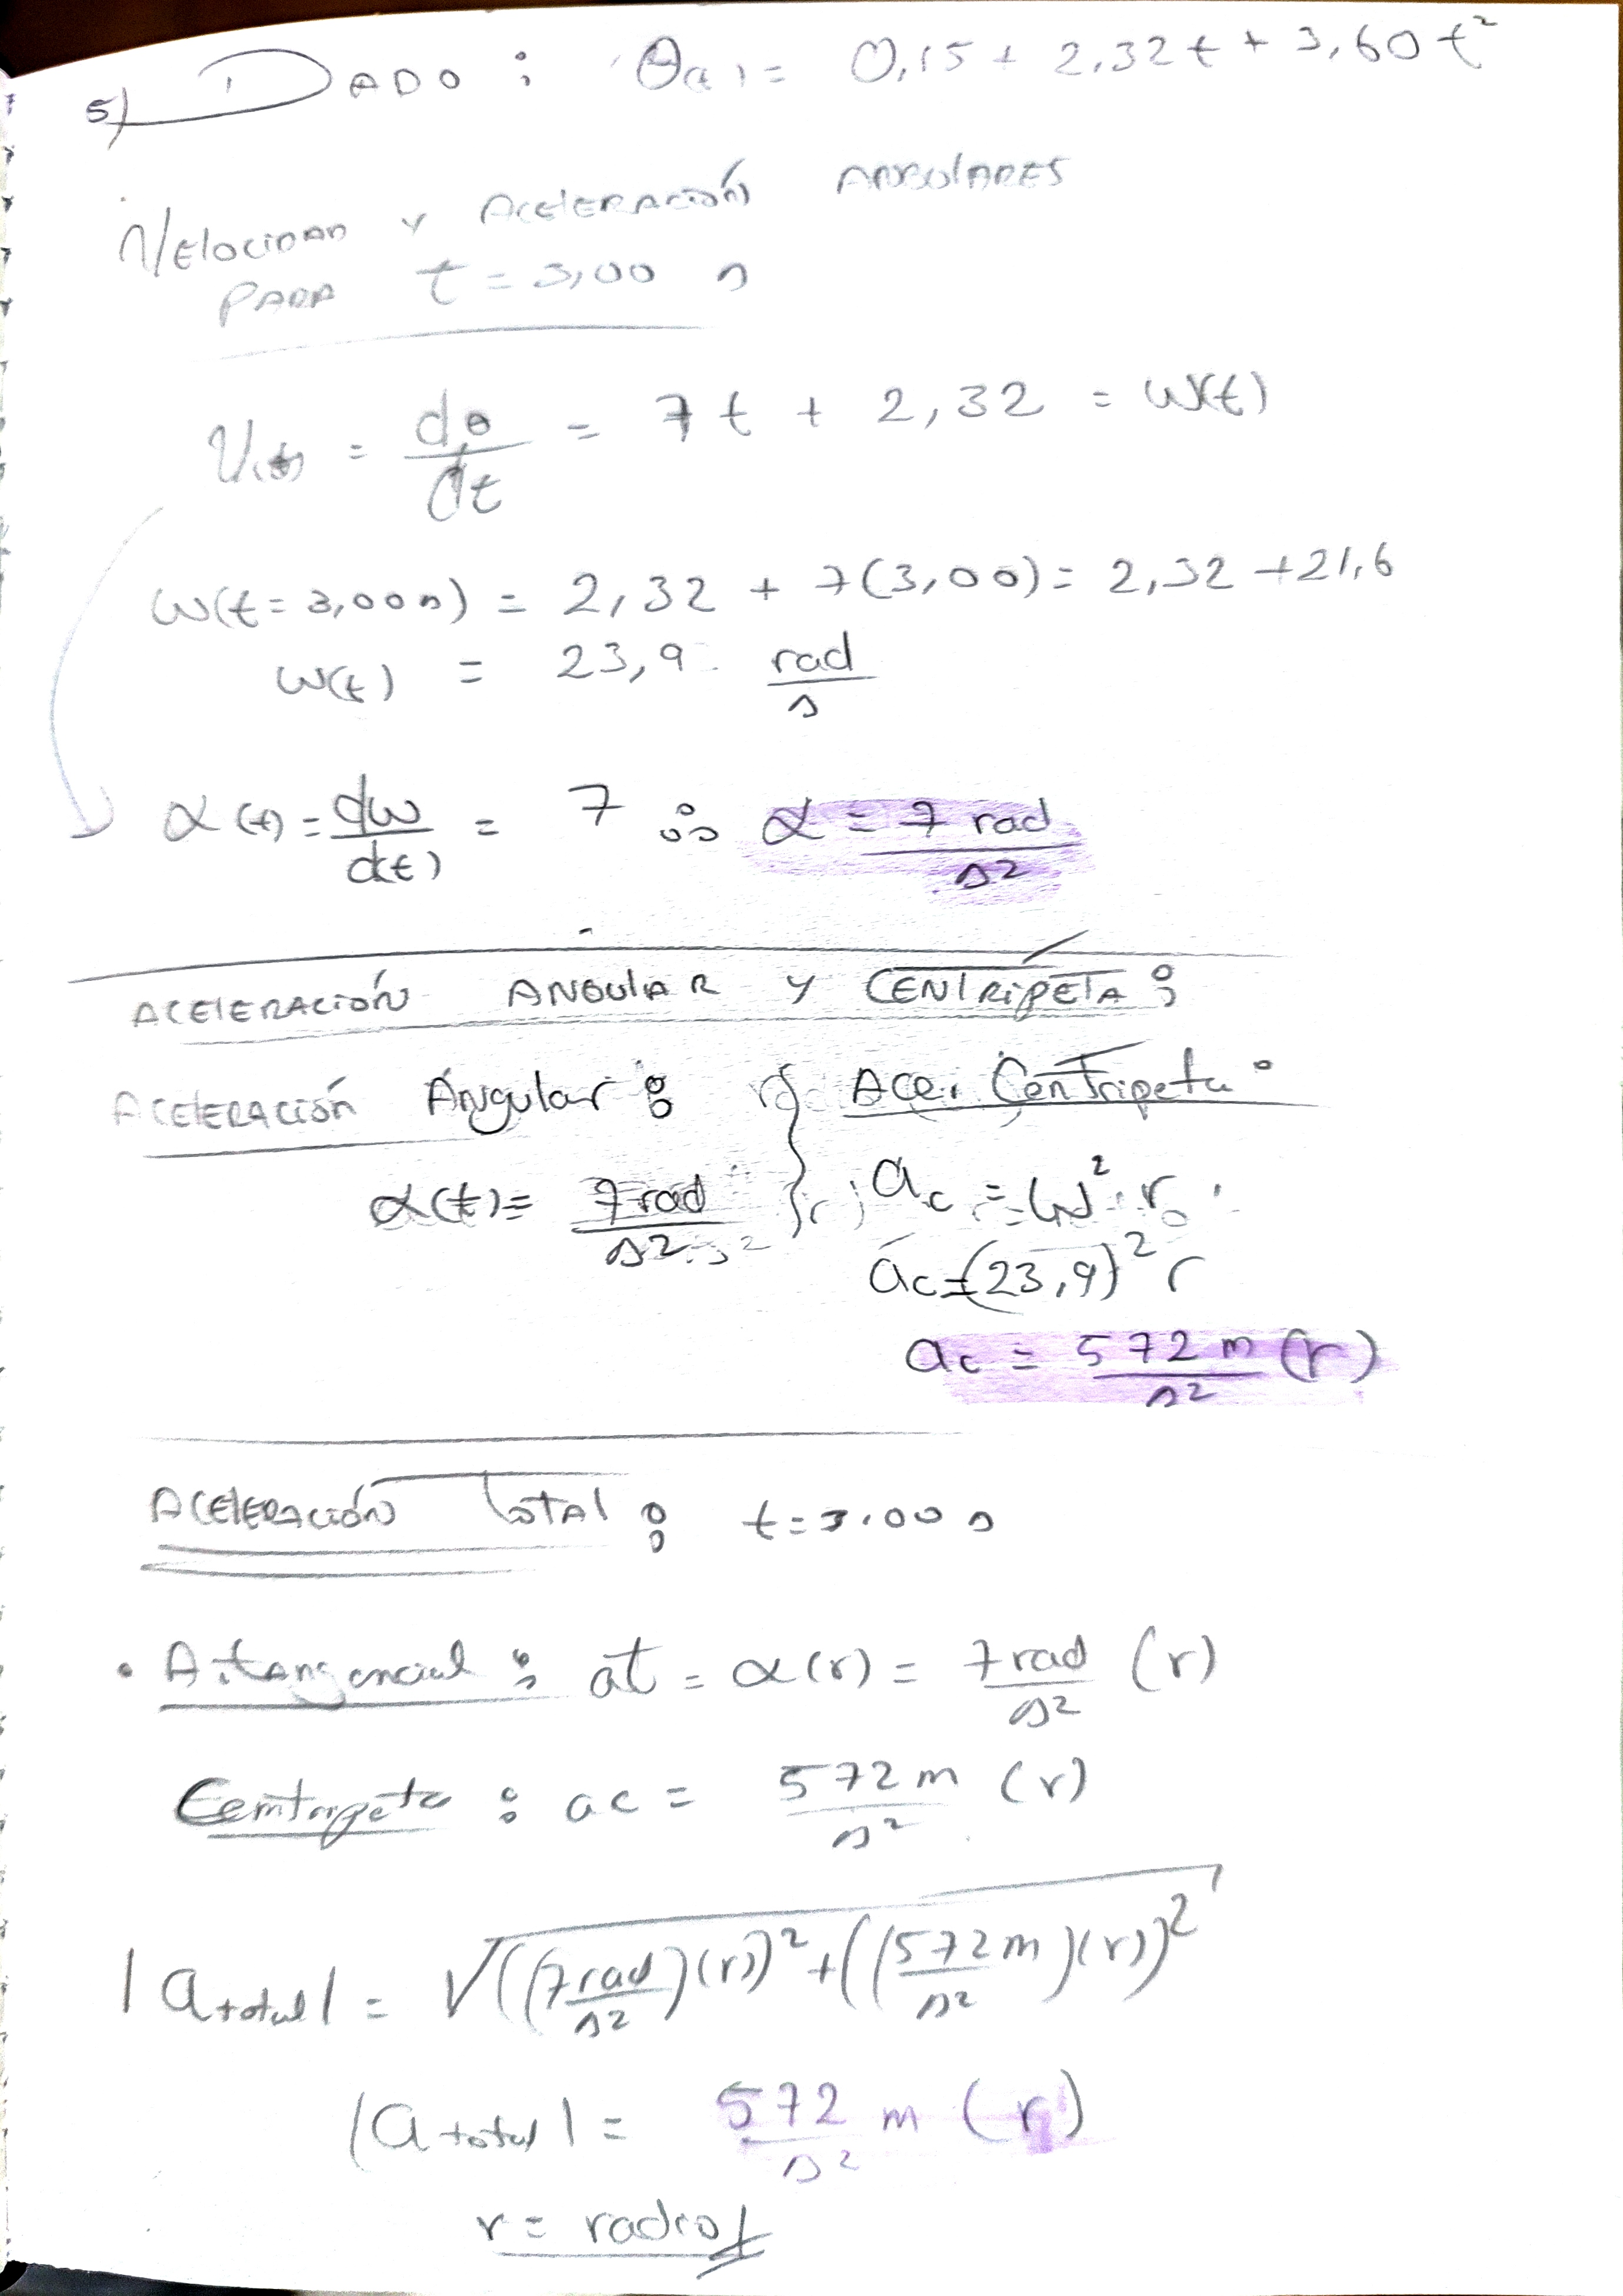
\includegraphics[width=0.9\textwidth]{assets/5.jpg}
  \label{fig:example_image5}
\end{figure}


\end{document}